%%%%%%%%%%%%%%%%%%%%%%%%%%%%%%%%%%%%
% Slide options
%%%%%%%%%%%%%%%%%%%%%%%%%%%%%%%%%%%%

% Option 1: Slides with solutions

\documentclass[slidestop,compress,mathserif]{beamer}
\newcommand{\soln}[1]{\textit{#1}}
\newcommand{\solnGr}[1]{#1}

% Option 2: Handouts without solutions

%\documentclass[11pt,containsverbatim,handout]{beamer}
%\usepackage{pgfpages}
%\pgfpagesuselayout{4 on 1}[letterpaper,landscape,border shrink=5mm]
%\newcommand{\soln}[1]{ }
%\newcommand{\solnGr}{ }

%%%%%%%%%%%%%%%%%%%%%%%%%%%%%%%%%%%%
% Style
%%%%%%%%%%%%%%%%%%%%%%%%%%%%%%%%%%%%

\input{../../lec_style.tex}
 

%%%%%%%%%%%%%%%%%%%%%%%%%%%%%%%%%%%%
% Preamble
%%%%%%%%%%%%%%%%%%%%%%%%%%%%%%%%%%%%

\title[Lecture 1]{MA213: Lecture 1}
\subtitle{Module 1: Exploratory Data Analysis and Study Design}
\author{OpenIntro Statistics, 4th Edition}
\institute{$\:$ \\ {\footnotesize Based on slides developed by Mine \c{C}etinkaya-Rundel of OpenIntro. \\
The slides may be copied, edited, and/or shared via the \webLink{http://creativecommons.org/licenses/by-sa/3.0/us/}{CC BY-SA license.} \\
Some images may be included under fair use guidelines (educational purposes).}}
\date{}

%%%%%%%%%%%%%%%%%%%%%%%%%%%%%%%%%%%%
% Begin document
%%%%%%%%%%%%%%%%%%%%%%%%%%%%%%%%%%%%

\begin{document}


%%%%%%%%%%%%%%%%%%%%%%%%%%%%%%%%%%%%
% Title page
%%%%%%%%%%%%%%%%%%%%%%%%%%%%%%%%%%%%

{
\addtocounter{framenumber}{-1} 
{\removepagenumbers 
\usebackgroundtemplate{\includegraphics[width=\paperwidth]{../../OpenIntro_Grid_4_3-01.jpg}}
\begin{frame}

\hfill \includegraphics[width=20mm]{../../oiLogo_highres}

\titlepage

\end{frame}
}
}

%%%%%%%%%%%%%%%%%%%%%%%%%%%%%%%%%%%%
% Sections
%%%%%%%%%%%%%%%%%%%%%%%%%%%%%%%%%%%%

%%%%%%%%%%%%%%%%%%%%%%%%%%%%%%%%%%%%
\section{Course Introduction}
%%%%%%%%%%%%%%%%%%%%%%%%%%%%%%%%%%%%

%%%%%%%%%%%%%%%%%%%%%%%%%%%%%%%%%%%
% Welcome
\begin{frame}
	\frametitle{Welcome to MA213: Basic Probability and Statistics}
	This is a newly redesigned course!
	\begin{itemize}
		\item \hl{We tried to design the course to be} accessible, engaging, and relevant.
		\item \hl{We want you to feel} connected to the course as a community and supported in your learning.
		\item \hl{We hope you will take away}
		\begin{itemize}
			\item A conceptual understanding of randomness and variability
			\item Practical skills for analyzing and interpreting data
			\item Confidence in your ability to work with data
			\item An appreciation for the beauty of statistics!
		\end{itemize}
		\item \hl{We will need your help} to make this course a success!
	\end{itemize}
\end{frame}

%%%%%%%%%%%%%%%%%%%%%%%%%%%%%%%%%%%
% People
\begin{frame}
	\frametitle{People}
	\begin{itemize}
		\item \hl{Instructor:} Prof. Emily Stephen
		\item \hl{Labs:} Dr. Yongho Lim
		\item \hl{Graduate Teaching Fellows (TFs):} 
		\begin{itemize}
			\item Matt Broe (Discussions)
			\item James Zheng Yang (Discussions)
			\item Matt Ludwig (Labs)
		\end{itemize}
		\item \hl{Undergraduate Learning Assistants (LAs):}
		\begin{itemize}
			\item Yao Lu
			\item Jack Hincks
		\end{itemize}
	\end{itemize}

	See the Syllabus for office hours and contact info
\end{frame}

%%%%%%%%%%%%%%%%%%%%%%%%%%%%%%%%%%%
% Logistics
\begin{frame}
	\frametitle{Class Logistics}
	\begin{itemize}
		\item \hl{Lectures}: Mon, Wed, Fri 11:15am-12:05pm
		\begin{itemize}
			\item Please bring a laptop or tablet for in-class activities
			\item Will be recorded
		\end{itemize}
		\item \hl{Labs}: Fridays
		\begin{itemize}
			\item Check your schedule for your time and location
			\item Start this week!
		\end{itemize}
		\item \hl{Discussions}: Once a week
		\begin{itemize}
			\item Check your schedule for your time and location
			\item Start next week!
		\end{itemize}
	\end{itemize}
\end{frame}

%%%%%%%%%%%%%%%%%%%%%%%%%%%%%%%%%%%
% Course Webpage

\begin{frame}
	\frametitle{Course Webpage} 
	\begin{itemize}
		\item \hl{Course website (Blackboard):} \url{https://learn.bu.edu} \\
		(Log in with your BU credentials)
		\item \hl{What's there:}
		\begin{itemize}
			\item Announcements
			\item Course documents: \textbf{Syllabus} (with Office Hours, GenAI policy, and Calendar), Learning Objectives
			\item Links to Textbook, Edfinity, Gradescope
			\item Course Forum
			\item Lecture slides and videos
			\item Lab materials
			\item Your gradebook
		\end{itemize}
	\end{itemize}	
\end{frame}

%%%%%%%%%%%%%%%%%%%%%%%%%%%%%%%%%%%
% Textbook

\begin{frame}
	\frametitle{Textbook: OpenIntro}
	\begin{columns}
		\column{0.6\textwidth}
		\begin{minipage}[t]{\linewidth}
		\vspace{0pt}
			\hl{OpenIntro Statistics}, 4th Edition \\
			David Diez, Mine \c{C}etinkaya-Rundel, and Christopher Barr \\
			\\
			\webLink{https://www.openintro.org/book/os/}{https://www.openintro.org/book/os/} \\
			\\
			Free download as PDF or \$25 for print copy
		\end{minipage}
		\column{0.4\textwidth}
		\begin{minipage}[t]{\linewidth}
		\vspace{0pt}
		\centering
		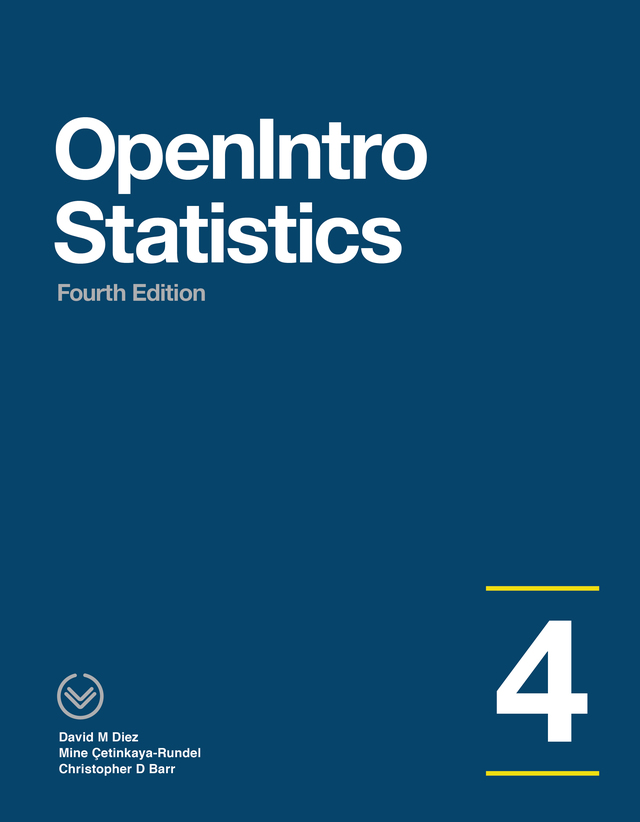
\includegraphics[width=0.9\columnwidth]{figures/openintro_cover.jpeg}
		\end{minipage}
	\end{columns}
\end{frame}

%%%%%%%%%%%%%%%%%%%%%%%%%%%%%%%%%%%
% Edfinity

\begin{frame}
	\frametitle{Edfinity} 
	We will use a platform called \hl{Edfinity} for \hl{in-class activities} and weekly \hl{homeworks}
	\begin{itemize}
		\item Access through the link on the course website
		\item Has interactive questions, optional support, and immediate feedback
		\item Homework grades and lecture participation will be synced with Blackboard
		\item Will cost \$40 for the semester
	\end{itemize}
\end{frame}

%%%%%%%%%%%%%%%%%%%%%%%%%%%%%%%%%%%
% Labs

\begin{frame}
	\frametitle{Labs} 
	Led by Yongho Lim, with support from TFs and LAs
	\begin{itemize}
		\item \hl{Weekly labs} on Fridays, starting this week
		\item \hl{Skills labs}
		\begin{itemize}
			\item Work in pairs
			\item Analyze data and run simulations in R
			\item Post-lab questions to be submitted on Gradescope
		\end{itemize}
		\item \hl{Lab projects}
		\begin{itemize}
			\item Work in groups to explore real data
			\item Project 1: Data analysis video presentation
			\item Project 2: Statistical report
		\end{itemize}
	\end{itemize}
	Please review the Lab 1 materials before your lab session!
\end{frame}

%%%%%%%%%%%%%%%%%%%%%%%%%%%%%%%%%%%
% Assignments and Grading Structure

\begin{frame}
	\frametitle{Assignments}
	\begin{itemize}
		\item 12 Weekly Edfinity \hl{homeworks}
		\begin{itemize}
			\item Due Mondays at 3:00pm
			\item Low-stakes, graded for completion
			\item Can revise and resubmit for full credit
			\item \hl{Homework 1} due Monday
		\end{itemize} 
		\item 5 \hl{Quizzes} 
		\begin{itemize}
			\item In discussion sections, see calendar in Syllabus
			\item 20 Core Learning Objectives, 11 Auxiliary Learning Objectives
			\item 5-6 written problems, graded pass / almost pass / not yet
			\item Can \textbf{qualify} to retake 3 quizzes at the end of the semester (details later)
		\end{itemize}
		\item 7 \hl{Skills Labs}
		\item 2 \hl{Lab Projects}
	\end{itemize}
\end{frame}

\begin{frame}
	\frametitle{Grading Structure}
	\begin{table}[ht]
	\centering
	\small
	\begin{tabular}{|l|c|c|c|}
	\hline
	 & \textbf{A} & \textbf{B} & \textbf{C} \\
	\hline
	Homeworks & 12/12 complete & 11/12 complete & 10/12 complete \\
	\hline
	Quizzes (Core) & 19/20 passed & 16/20 passed & 12/20 passed \\
	\hline
	Quizzes (Aux) & 9/11 passed & 6/11 passed & 0/11 passed \\
	\hline
	Skills Labs & 7/7 passed & Labs 1-6 passed & Labs 1-6 passed \\
	\hline
	Lab Projects & 2 satisfactory & 2 satisfactory & 2 satisfactory \\
	\hline
	Lectures & $<$5 missed & $<$9 missed & $<$15 missed \\
	\hline
	\end{tabular}
	\end{table}

	\hl{Additional factors:}
	\begin{itemize}
		\item Grades between letter grades will be determined by how close you are to the next letter grade
		\item Each ``unsatisfactory'' project will drop your course grade by a third of a letter grade (e.g. B to B-)
	\end{itemize}
\end{frame}

%%%%%%%%%%%%%%%%%%%%%%%%%%%%%%%%%%%
% Learning Objectives

\begin{frame}
	\frametitle{Learning Objectives}

	\textcolor{red}{Core} Learning Objectives \\
	\textcolor{blue}{Auxiliary} Learning Objectives \\

	\vspace{10pt}
	Module 1: Exploratory Data Analysis and Study Design \\(Chapters 1-2)
	\begin{enumerate}
		\item (\textcolor{red}{core}, Q1) Classify and analyze variables 
		\item (\textcolor{red}{core}, Q1) Evaluate Study Design and Its Implications 
		\item (\textcolor{red}{core}, Labs) Use R for Data Management and Exploration
		\item (\textcolor{red}{core}, Q1) Visualize and Describe Data Distributions 
		\item (\textcolor{blue}{aux}, Q1) Conduct Hypothesis Testing Using Simulation 
	\end{enumerate}
	See the Syllabus and Learning Objectives document for details
\end{frame}

\begin{frame}
	\frametitle{Learning Objectives}
	Module 6: Global module (\textcolor{red}{core})
	\begin{enumerate}
		\item (Projects) I can carry out a complete, reproducible statistical workflow in R using the inference methods from the course  
		\item (Q1, Q4) Given R code for a statistical analysis, I can explain what it does and why, and identify both programmatic and statistical errors 
		\item (Quizzes) When solving probability and statistics problems, I can support my answers by writing out the steps using the notation and conventions of statistical exposition  
		\item (Projects) I can recognize whether a statistical workflow is appropriate for the given data and data analysis goals, and explain the results of a statistical analysis to stakeholders
	\end{enumerate}
\end{frame}

%%%%%%%%%%%%%%%%%%%%%%%%%%%%%%%%%%%

\begin{frame}
	\frametitle{Class Policies} 
	\begin{itemize}
		\item \hl{Attendance and participation:} 
		\begin{itemize}
			\item Expected to attend all lectures, labs, and discussions. 
			\item In-class activities and participation will be part of your grade.
			\item Email the instructor or your TF if you need to miss class/discussion/lab
		\end{itemize}
		\item \hl{Academic integrity:} 
		\begin{itemize}
			\item All work must be your own. 
			\item Collaboration is allowed on homeworks and labs/projects, but \textbf{not on quizzes}. 
			\item See Syllabus for details.
		\end{itemize}
		\item \hl{Use of Generative AI tools (e.g. ChatGPT):}
		\begin{itemize}
			\item Quizzes: \textbf{Not allowed}.
			\item Homeworks: Use at your own discretion
			\item Labs/Projects: Allowed for \textbf{specific uses} with \textbf{proper documentation}.
			\item See GenAI policy in the Syllabus for details.
		\end{itemize}
	\end{itemize}
\end{frame}

%%%%%%%%%%%%%%%%%%%%%%%%%%%%%%%%%%%
% Calendar
\begin{frame}
	\frametitle{Course Calendar} 
    \begin{center}
        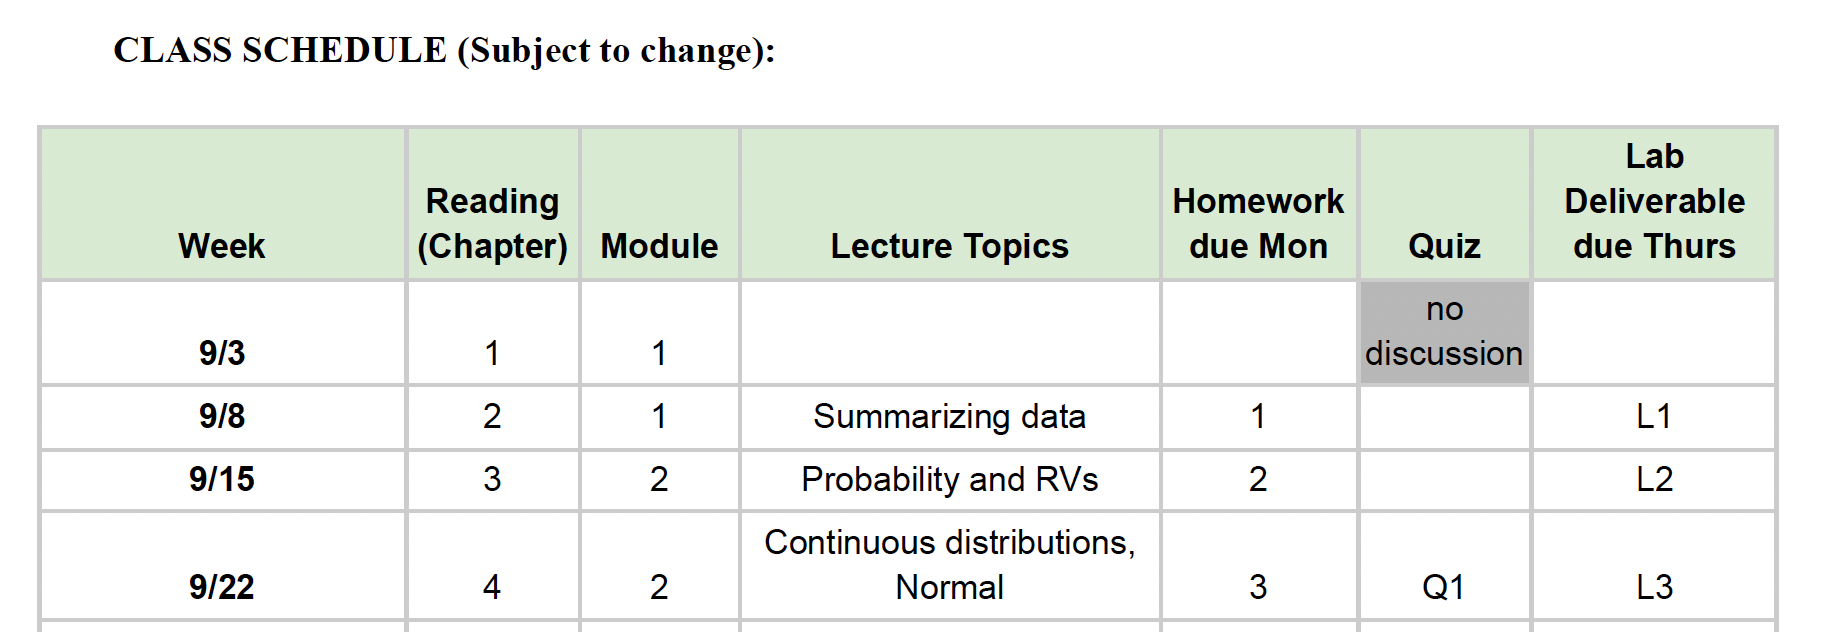
\includegraphics[width=0.95\textwidth]{figures/2025_Calendar.png}
    \end{center}
	\begin{itemize}
		\item \hl{See the Syllabus} for the full calendar (subject to change)
		\item \hl{Edfinity Homeworks:} Due Monday at 3:00pm
		\item \hl{Quizzes:} In discussion sections
		\item \hl{Skills Labs:} Due the following Thursday at 10:00pm
		\item \hl{Lab Projects:} See Syllabus for deadlines
	\end{itemize}
\end{frame}
%%%%%%%%%%%%%%%%%%%%%%%%%%%%%%%%%%%

%%%%%%%%%%%%%%%%%%%%%%%%%%%%%%%%%%%%
\section{A Case Study}
%%%%%%%%%%%%%%%%%%%%%%%%%%%%%%%%%%%%

\begin{frame}
\frametitle{Treating Chronic Fatigue Syndrome}

\begin{itemize}

\item Objective: Evaluate the effectiveness of cognitive-behavior therapy for chronic fatigue syndrome.

\item Participant pool: 142 patients who were recruited from referrals by primary care physicians and consultants to a hospital clinic specializing in chronic fatigue syndrome.

\item Actual participants: Only 60 of the 142 referred patients entered the study. Some were excluded because they didn't meet the diagnostic criteria, some had other health issues, and some refused to be a part of the study.

\end{itemize}

\ct{Deale et. al. \textit{Cognitive behavior therapy for chronic fatigue syndrome: A randomized controlled trial}. The American Journal of Psychiatry 154.3 (1997).}

\end{frame}

%%%%%%%%%%%%%%%%%%%%%%%%%%%%%%%%%%%%

\begin{frame}
\frametitle{Study design}

\begin{itemize}

\item Patients randomly assigned to treatment and control groups, 30 patients in each group:
\begin{itemize}
\item \hl{Treatment}: Cognitive behavior therapy -- collaborative, educative, and with a behavioral emphasis. Patients were instructed on how activity could be increased steadily and safely without exacerbating symptoms.
\item \hl{Control:} Relaxation -- No advice was given about how activity could be increased. Instead progressive muscle relaxation, visualization, and rapid relaxation skills were taught.
\end{itemize}

\end{itemize}

\end{frame}

%%%%%%%%%%%%%%%%%%%%%%%%%%%%%%%%%%%%

\begin{frame}
\frametitle{Results}

The table below shows the distribution of patients with good outcomes at 6-month follow-up. Note that 7 patients dropped out of the study: 3 from the treatment and 4 from the control group.

\begin{center}
\begin{tabular}{ll  cc c} 
			&				& \multicolumn{2}{c}{\textit{Good outcome}} \\
\cline{3-4}
			&							& Yes 	& No 	& Total	\\
\cline{2-5}
							&Treatment 	& 19	 	& 8		& 27 	\\
\raisebox{1.5ex}[0pt]{\textit{Group}}	&Control		& 5	 	& 21	 	& 26 \\
\cline{2-5}
							&Total		& 24		& 29		& 53
\end{tabular}
\end{center}

\pause

\begin{itemize}

\item Proportion with good outcomes in treatment group:
\[ 19 / 27 \approx 0.70 \rightarrow 70\% \]

\pause

\item Proportion with good outcomes in control group:
\[ 5 / 26 \approx 0.19 \rightarrow 19\% \]

\end{itemize}

\end{frame}

%%%%%%%%%%%%%%%%%%%%%%%%%%%%%%%%%%%
% Think/pair/share: Do the data show a "real" difference between groups? Are the results generalizable?
\begin{frame}
	\frametitle{Think/Pair/Share: Case Study}
	\begin{itemize}
		\item \textbf{Think (2 mins):} Do the data show a ``real'' difference between groups? Are the results generalizable?
		\item \textbf{Pair (3 mins):} Discuss with the person sitting next to you.
		\item \textbf{Share (3 mins):} Share your thoughts in the class discussion forum.
	\end{itemize}

	The ``Lecture 1 Think/Pair/Share'' discussion board is under the \textit{Discussions} tab in the course website, in the Lectures Folder. 
\end{frame}

%%%%%%%%%%%%%%%%%%%%%%%%%%%%%%%%%%%%
\begin{frame}
\frametitle{Understanding the results}

\dq{Do the data show a ``real" difference between the groups?}


\begin{itemize}

\item Suppose you flip a coin 100 times. While the chance a coin lands heads in any given coin flip is 50\%, we probably won't observe exactly 50 heads. This type of fluctuation is part of almost any type of data generating process.

\item The observed difference between the two groups (70 - 19 = 51\%) may be real, or may be due to natural variation.

\item Since the difference is quite large, it is more believable that the difference is real.

\item We need statistical tools to determine if the difference is so large that we should reject the notion that it was due to chance.

\end{itemize}

\end{frame}

%%%%%%%%%%%%%%%%%%%%%%%%%%%%%%%%%%%%

\begin{frame}
\frametitle{Generalizing the results}

\dq{Are the results of this study generalizable to all patients with chronic fatigue syndrome?}


These patients had specific characteristics and volunteered to be a part of this study, therefore they may not be representative of all patients with chronic fatigue syndrome. While we cannot immediately generalize the results to all patients, this first study is encouraging. The method works for patients with some narrow set of characteristics, and that gives hope that it will work, at least to some degree, with other patients.


\end{frame}

%%%%%%%%%%%%%%%%%%%%%%%%%%%%%%%%%%%
% Big picture of statistics 
% https://stats.libretexts.org/Bookshelves/Applied_Statistics/Biostatistics_-_Open_Learning_Textbook/Preliminaries/The_Big_Picture
% https://creativecommons.org/licenses/by-nc-sa/4.0/

\begin{frame}
    \frametitle{Big Picture of Statistics}
    \begin{center}
        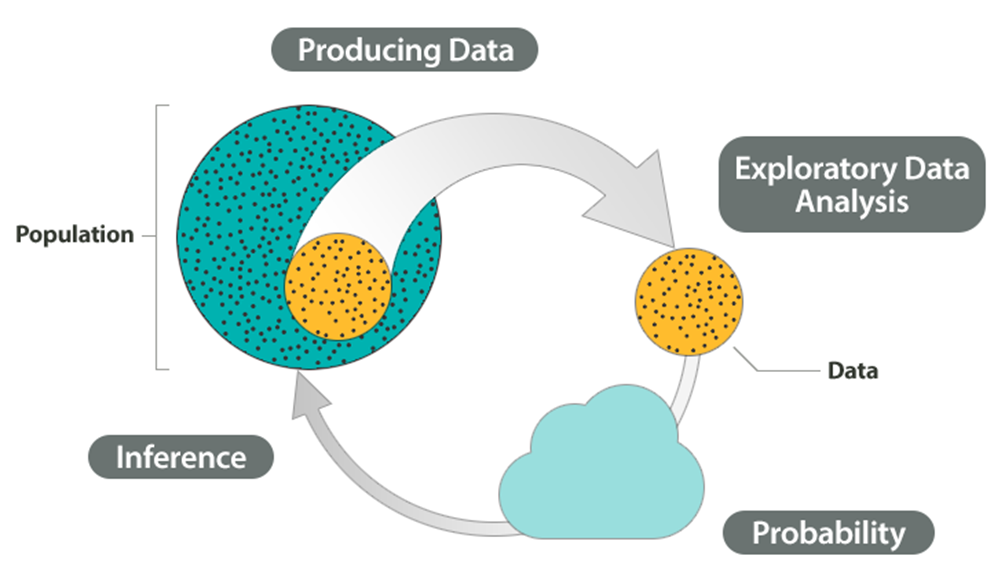
\includegraphics[width=0.95\textwidth]{figures/BigPicture1.png}
    \end{center}
    \vspace{0.5em}
    \footnotesize
    Credit: \href{https://stats.libretexts.org/Bookshelves/Applied_Statistics/Biostatistics_-_Open_Learning_Textbook/Preliminaries/The_Big_Picture}{LibreTexts}
    \\
    Licensed under \href{https://creativecommons.org/licenses/by-nc-sa/4.0/}{CC BY-NC-SA 4.0}
\end{frame}

\begin{frame}
    \frametitle{Big Picture of Statistics}
    \begin{center}
        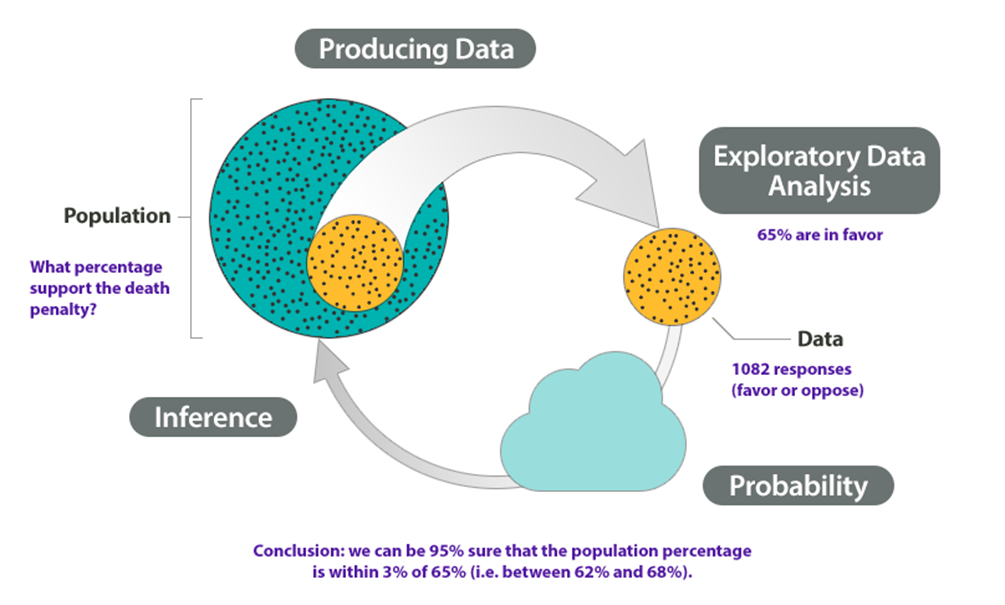
\includegraphics[width=0.95\textwidth]{figures/BigPicture2.png}
    \end{center}
    \vspace{0.5em}
    \footnotesize
    Credit: \href{https://stats.libretexts.org/Bookshelves/Applied_Statistics/Biostatistics_-_Open_Learning_Textbook/Preliminaries/The_Big_Picture}{LibreTexts}
    \\
    Licensed under \href{https://creativecommons.org/licenses/by-nc-sa/4.0/}{CC BY-NC-SA 4.0}
\end{frame}
%%%%%%%%%%%%%%%%%%%%%%%%%%%%%%%%%%%%

% If time, start data basics slides  % TODO

%%%%%%%%%%%%%%%%%%%%%%%%%%%%%%%%%%%

\begin{frame}
	\frametitle{Edfinity Classroom Survey} 

	Please take the Edfinity ``classroom survey'' poll to get data for next Lecture.

	\begin{itemize}
		\item Follow the Edfinity link on the course website
		\item If you haven't already, you will be prompted to pay and enroll in the course
		\item The survey should take 2-3 minutes
		\item Will be used to illustrate data basics in the next lecture
	\end{itemize}
\end{frame}

%%%%%%%%%%%%%%%%%%%%%%%%%%%%%%%%%%%

% Final announcements 

%%%%%%%%%%%%%%%%%%%%%%%%%%%%%%%%%%%%
% Recap/Agenda 
%%%%%%%%%%%%%%%%%%%%%%%%%%%%%%%%%%%%
% TODO better formatting
\begin{frame}
    \frametitle{Module 1: Exploratory Data Analysis and Study Design}
    \begin{itemize}
        % \item \hl{This time: }Course introduction
        \item \hl{Reading: }Chapter 1 for next time
        \item \hl{Deadlines/Announcements: }
        \begin{itemize}
            \item See/email me (estephen@bu.edu) for any registration issues
            \item Edfinity classroom survey by lecture on Friday \\
            (if you haven't done it yet)
            \item Labs start this week (Friday)
            \item Discussions start next week
            \item Edfinity Homework 1 due on Monday
        \end{itemize}
    \end{itemize}
    
\end{frame}
    

%%%%%%%%%%%%%%%%%%%%%%%%%%%%%%%%%%%

%%%%%%%%%%%%%%%%%%%%%%%%%%%%%%%%%%%%
% End document
%%%%%%%%%%%%%%%%%%%%%%%%%%%%%%%%%%%%

\end{document}